%! TeX program = lualatex
\documentclass[12pt,a4paper]{article}

\usepackage[nil]{babel}
\usepackage{unicode-math}
\usepackage[svgnames]{xcolor}
\usepackage{lmodern}
\usepackage{graphicx}
\usepackage{wrapfig}
\usepackage{float}
\usepackage{parskip}
\usepackage{enumitem}

\makeatother
\babelprovide[import=el, main, onchar=ids fonts]{greek} % can also do import=el-polyton
\babelprovide[import, onchar=ids fonts]{english}

\babelfont{rm}
          [Language=Default]{Liberation Sans}
\babelfont[english]{rm}
          [Language=Default]{Liberation Sans}
\babelfont{sf}
          [Language=Default]{Liberation Sans}
\babelfont{tt}
          [Language=Default]{Liberation Sans}

%Enter Title Here
\title{Use-cases-v0.1 \\ LibShare}
\author{\textbf{Ονόματα / ΑΜ / Έτος:} \\ Γρηγόρης Καπαδούκας / 1072484 / 4\textdegree \\ Χρήστος Μπεστητζάνος / 1072615 / 4\textdegree \\ Νικόλαος Αυγέρης / 1067508 / 5\textdegree \\ Περικλής Κοροντζής / 1072563 / 4\textdegree}

\begin{document}

\makeatletter
\begin{center}
	\LARGE{\@title} \\
	\pagebreak
	\begin{LARGE}\@author\end{LARGE} \\
\end{center}
\pagebreak

%Insert Body Here
\section{Use Case Diagram}

Το Use Case Diagram που φτιάξαμε αποτελεί το Σχήμα \ref{Use Case Diagram}. Για την καλύτερη και πιο λεπτομερή σχεδίαση, πολλά use cases τα οποία αποτελούν ένα use case παρακάτω στο κεφάλαιο \ref{Ροές των Use Cases}, εδώ έχουν αποτελέσει περισσότερα από ένα με σκοπό την καλύτερη ανάλυση της αλληλεπίδρασης μεταξύ των use cases.

Έτσι για παράδειγμα, το use case της "Αναζήτησης βιβλίων / χρήστη, αιτήσεων" στο κεφάλαιο \ref{Ροές των Use Cases} εδώ χωρίζεται σε "Αναζήτηση", "Αναζήτηση βιβλίου", "Αναζήτηση χρήστη" και "Αναζήτηση αίτησης", με σχέση γενίκευσης των τριών τελευταίων από το πρώτο. Επίσης τα use cases με σχέση extends μπορούν στο κεφάλαιο \ref{Ροές των Use Cases} να αναπαρασταθούν σε ένα use case, με ένδειξη της επιπλέον λειτουργικότητας σε εναλλακτική ροή. Με αυτόν τον τρόπο προσπαθούμε να αποφύγουνε να αναλύσουμε τετριμμένα use cases.

\begin{figure}[H]
	\makebox[\textwidth]{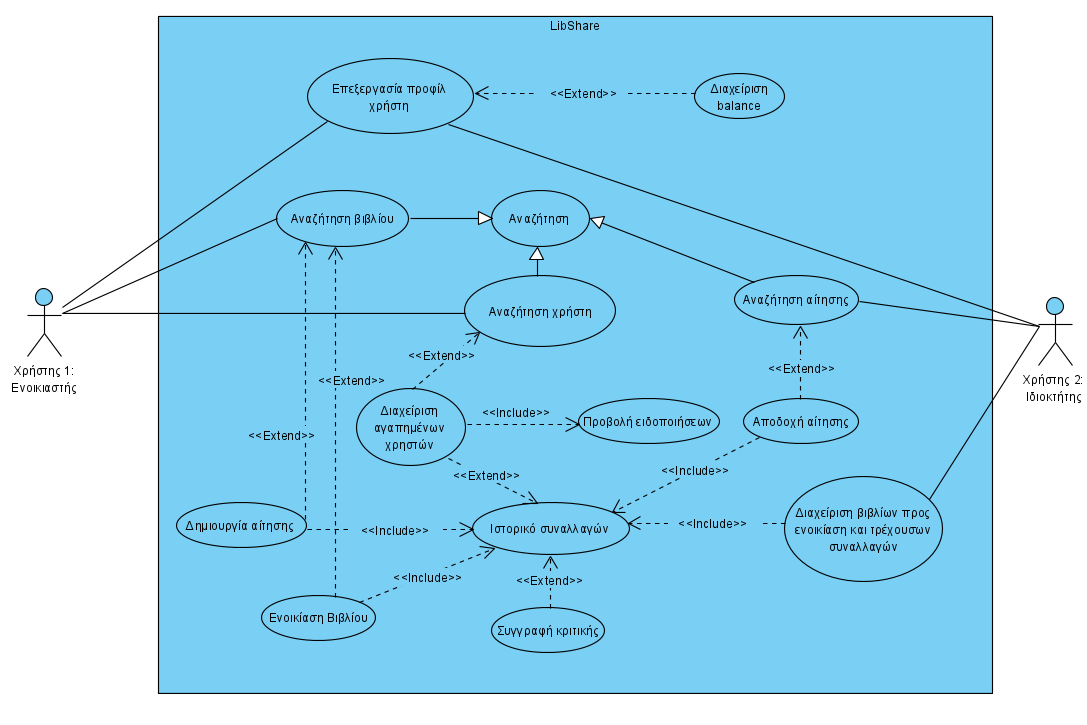
\includegraphics[width=\textwidth]{Use-case Diagram.png}}
	\caption{Use Case Diagram}
	\label{Use Case Diagram}
\end{figure}


\section{Ροές των Use Cases}
\label{Ροές των Use Cases}

\subsection{Αναζήτηση βιβλίων / χρήστη / αιτήσεων}

\subsubsection*{Βασική Ροή <<Αναζήτηση βιβλίων / χρήστη / αιτήσεων>>: Αναζήτηση βιβλίων:}
\begin{enumerate}
    \item Ο χρήστης επιλέγει φίλτρο αναζήτησης "βιβλία", με τύπο συναλλαγής "και τα δύο" (δηλαδή και από κοντά και ταχυδρομικώς) και εισάγει ένα κείμενο αναζήτησης (μπορεί να είναι και τίτλος βιβλίου και όνομα συγγραφέα).
        \label{Επιλογή τύπου αναζήτησης}
    \item Το σύστημα ελέγχει αν υπάρχουν διαθέσιμα βιβλία προς ενοικίαση που να πληρούν το κείμενο αναζήτησης και το τύπο συναλλαγής και βλέπει ότι υπάρχουν.
        \label{Ύπαρξη βιβλίου}
    \item Το σύστημα δείχνει τη λίστα με τα διαθέσιμα βιβλία στον χρήστη, περιέχοντας τους πλήρεις τίτλους, το όνομα συγγραφέα, τον εκδοτικό οίκο και έτος τύπωσης.
    \item Ο χρήστης επιλέγει ένα από τα βιβλία.
    \item Το σύστημα φορτώνει τη λίστα των ιδιοκτητών που προσφέρουν το βιβλίο που επιλέχθηκε και την προβάλλει στον χρήστη, μαζί με την τιμή του βιβλίου ανά μέρα, την πόλη που μένει ο κάθε χρήστης, το σκορ του (που προκύπτει από τα ratings άλλων χρηστών) και κουμπί που του επιτρέπει να κάνει αίτηση ενοικίασης του βιβλίου στον χρήστη αυτόν.
\end{enumerate}

\subsubsection*{Εναλλακτική Ροή 1: Αναζήτηση χρήστη - Αυτός υπάρχει:}
\begin{enumerate}
    \item[\ref{Επιλογή τύπου αναζήτησης}.α.1.] Ο χρήστης επιλέγει φίλτρο αναζήτησης "χρήστης" και εισάγει ένα κείμενο αναζήτησης (το username του χρήστη που αναζητεί).
    \item[\ref{Επιλογή τύπου αναζήτησης}.α.2.] Το σύστημα ελέγχει αν υπάρχει άλλος χρήστης με το όνομα που ζήτησε ο χρήστης και βλέπει ότι υπάρχει.
    \item[\ref{Επιλογή τύπου αναζήτησης}.α.3.] Το σύστημα προβάλλει στον χρήστη το προφίλ του χρήστη που αναζήτησε, δηλαδή το username, το rating του, την τοποθεσία που μένει και το description που έχει ορίσει για τον λογαριασμό του. Επίσης προβάλλει ένα κουμπί προσθήκης χρήστη στη λίστα των αγαπημένων (το οποίο χρησιμοποιείται για το use case των notifications και αγαπημένων).
\end{enumerate}

\subsubsection*{Εναλλακτική Ροή 2: Αναζήτηση χρήστη - Αυτός δεν υπάρχει:}
\begin{enumerate}
    \item[\ref{Επιλογή τύπου αναζήτησης}.α.2.1.] Το σύστημα ελέγχει αν υπάρχει άλλος χρήστης με το όνομα που ζήτησε ο χρήστης και βλέπει ότι δεν υπάρχει.
    \item[\ref{Επιλογή τύπου αναζήτησης}.α.2.2.] Το σύστημα ενημερώνει τον χρήστη ότι ο χρήστης που αναζητεί δεν υπάρχει.
\end{enumerate}

\subsubsection*{Εναλλακτική Ροή 3: Αναζήτηση αίτησης - Αυτή υπάρχει:}
\begin{enumerate}
    \item[\ref{Επιλογή τύπου αναζήτησης}.β.1.] Ο χρήστης επιλέγει φίλτρο αναζήτησης "αιτήσεις", με τύπο συναλλαγής "και τα δύο", και εισάγει ένα κείμενο αναζήτησης (το όνομα του βιβλίου για το οποίο αναζητά αν υπάρχουν αιτήσεις).
    \item[\ref{Επιλογή τύπου αναζήτησης}.β.2.] Το σύστημα ελέγχει αν υπάρχει αίτηση που να πληρεί τα κριτήρια αναζήτησης που ζήτησε ο χρήστης και διαπιστώνει ότι υπάρχει.
    \item[\ref{Επιλογή τύπου αναζήτησης}.β.3.] Το σύστημα δείχνει τη λίστα με τα βιβλία για τα οποία υπάρχουν αιτήσεις που πληρούν τα κριτήρια αναζήτησης στον χρήστη, περιέχοντας τους πλήρεις τίτλους, το όνομα συγγραφέα, τον εκδοτικό οίκο και έτος τύπωσης.
    \item[\ref{Επιλογή τύπου αναζήτησης}.β.4.] Ο χρήστης επιλέγει ένα από τα βιβλία.
    \item[\ref{Επιλογή τύπου αναζήτησης}.β.5.] Το σύστημα φορτώνει τη λίστα των χρηστών που έχουν κάνει αίτηση για το βιβλίο που επιλέχθηκε και την προβάλλει στον χρήστη, μαζί με την τιμή που προτίθενται να πληρώσει ο κάθε χρήστης για το βιβλίο ανά μέρα, την πόλη που μένει ο καθένας, το σκορ τους και κουμπί που του επιτρέπει να κάνει αποδοχή της αίτησης.
\end{enumerate}

\subsubsection*{Εναλλακτική Ροή 4: Αναζήτηση αίτησης - Αυτή δεν υπάρχει:}
\begin{enumerate}
    \item[\ref{Επιλογή τύπου αναζήτησης}.β.2.1.] Το σύστημα ελέγχει αν υπάρχει αίτηση για το βιβλίο που αναζήτησε ο χρήστης και διαπιστώνει ότι δεν υπάρχει.
    \item[\ref{Επιλογή τύπου αναζήτησης}.β.2.2.] Το σύστημα ενημερώνει τον χρήστη ότι δεν υπάρχει αίτηση που να πληρεί τα κριτήρια αναζήτησης.
\end{enumerate}

\subsubsection*{Εναλλακτική Ροή 5: Αναζήτηση βιβλίου - Μόνο από κοντά:}
\begin{enumerate}
    \item[\ref{Επιλογή τύπου αναζήτησης}.γ.1.] Ο χρήστης επιλέγει φίλτρο αναζήτησης "βιβλία", με τύπο συναλλαγής "μόνο από κοντά" και εισάγει ένα κείμενο αναζήτησης (μπορεί να είναι και τίτλος βιβλίου και όνομα συγγραφέα).
    \item[\ref{Επιλογή τύπου αναζήτησης}.γ.2.] Η περίπτωση χρήσης συνεχίζεται από το βήμα \ref{Ύπαρξη βιβλίου} της βασικής ροής.
\end{enumerate}

\subsubsection*{Εναλλακτική Ροή 6: Αναζήτηση βιβλίου - Μόνο ταχυδρομικώς:}
\begin{enumerate}
    \item[\ref{Επιλογή τύπου αναζήτησης}.δ.1.] Ο χρήστης επιλέγει φίλτρο αναζήτησης "βιβλία", με τύπο συναλλαγής "μόνο ταχυδρομικώς" και εισάγει ένα κείμενο αναζήτησης (μπορεί να είναι και τίτλος βιβλίου και όνομα συγγραφέα).
    \item[\ref{Επιλογή τύπου αναζήτησης}.δ.2.] Η περίπτωση χρήσης συνεχίζεται από το βήμα \ref{Ύπαρξη βιβλίου} της βασικής ροής.
\end{enumerate}

\subsubsection*{Εναλλακτική Ροή 7: Αναζήτηση βιβλίου - Αυτό δεν υπάρχει:}
\begin{enumerate}
    \item[\ref{Ύπαρξη βιβλίου}.1.] Το σύστημα ελέγχει αν υπάρχουν διαθέσιμα βιβλία προς ενοικίαση που να πληρούν το κείμενο αναζήτησης και βλέπει ότι δεν υπάρχουν.
    \item[\ref{Ύπαρξη βιβλίου}.2.] Το σύστημα ενημερώνει τον χρήστη ότι δεν υπάρχουν διαθέσιμα βιβλία που να πληρούν τα κριτήρια αναζήτησης. 
\end{enumerate}

\subsubsection*{Εναλλακτική Ροή 8: Αναζήτηση αίτησης - Μόνο από κοντά:}
\begin{enumerate}
    \item[\ref{Επιλογή τύπου αναζήτησης}.β.1.α.1.] Ο χρήστης επιλέγει φίλτρο αναζήτησης "αιτήσεις", με τύπο συναλλαγής "μόνο από κοντά", και εισάγει ένα κείμενο αναζήτησης (το όνομα του βιβλίου για το οποίο αναζητά αν υπάρχουν αιτήσεις).
    \item[\ref{Επιλογή τύπου αναζήτησης}.β.1.α.2.] Η περίπτωση χρήσης συνεχίζεται από το βήμα 2.γ.1.2 της βασικής ροής.
\end{enumerate}

\subsubsection*{Εναλλακτική Ροή 9: Αναζήτηση αίτησης - Μόνο ταχυδρομικώς:}
\begin{enumerate}
    \item[\ref{Επιλογή τύπου αναζήτησης}.β.1.β.1.] Ο χρήστης επιλέγει φίλτρο αναζήτησης "αιτήσεις", με τύπο συναλλαγής "μόνο ταχυδρομικώς", και εισάγει ένα κείμενο αναζήτησης (το όνομα του βιβλίου για το οποίο αναζητά αν υπάρχουν αιτήσεις).
    \item[\ref{Επιλογή τύπου αναζήτησης}.β.1.β.2.] Η περίπτωση χρήσης συνεχίζεται από το βήμα 2.γ.1.2 της βασικής ροής.
\end{enumerate}


\subsection{Ενοικίαση βιβλίου από άλλο χρήστη}
\label{Rental Use Case}
\subsubsection*{Βασική Ροή <<Ενοικίαση βιβλίου από άλλο χρήστη>>: Συναλλαγή από κοντά:}
\begin{enumerate}
    \item Ο ενοικιαστής κάνει αίτηση ενοικίασης στον ιδιοκτήτη που επέλεξε για το βιβλίο που αναζήτησε, επιλέγοντας συναλλαγή από κοντά.
        \label{Επιλογή τρόπου συναλλαγής}
    \item Το σύστημα επιβεβαιώνει ότι ο ενοικιαστής έχει αρκετά χρήματα στο λογαριασμό του για να καλύψει το "ποσό ασφαλείας" που θα δεσμευτεί αργότερα από τον λογαριασμό του.
        \label{Έλεγχος ποσού ασφαλείας}
    \item Το σύστημα επιβεβαιώνει ότι η αίτηση ενοικίασης έχει γίνει αποδεκτή από τον ιδιοκτήτη.
        \label{Αποδοχή ή απόρριψη συναλλαγής}
    \item Το σύστημα εμφανίζει στοιχεία επικοινωνίας του ιδιοκτήτη στον ενοικιαστή.
    \item Ο ενοικιαστής, αφού βρεθεί με τον ιδιοκτήτη από κοντά και παραλάβει το βιβλίο, ενημερώνει το σύστημα ότι έχει κατοχή του βιβλίου. Ο ιδιοκτήτης επίσης ενημερώνει το σύστημα.
    \item Το σύστημα ελέγχει αν έλαβε ενημέρωση κατοχής του βιβλίου και από τον ενοικιαστή και από τον ιδιοκτήτη.
        \label {Δεν ενημερώνεται η κατοχή}
    \item Το σύστημα δεσμεύει "ποσό ασφαλείας" από τον λογαριασμό του ενοικιαστή, και αρχίζει να τον χρεώνει αυτόματα μέρα με τη μέρα.
        \label{Τέλος dispute resolved - Τέλος χρημάτων}
    \item Ο ενοικιαστής, αφού τελειώσει το βιβλίο, βρίσκεται πάλι με τον ιδιοκτήτη και του παραχωρεί το βιβλίο, έπειτα του οποίου ενημερώνουν και οι δύο το σύστημα ότι το βιβλίο έχει επιστραφεί.
        \label{Επιστροφή βιβλίου - Τέλος λεφτά δεν φτάνουν}
    \item Το σύστημα, αφού λάβει ενημέρωση επιστροφής βιβλίου και από τα δύο μέλη, σταματάει να χρεώνει τον ενοικιαστή και του επιστρέφει το "ποσό ασφαλείας".
        \label{Τέλος ενοικίασης}
\end{enumerate}

\subsubsection*{Εναλλακτική Ροή 1: Η συναλλαγή γίνεται ταχυδρομικώς:}
\begin{enumerate}
    \item[\ref{Επιλογή τρόπου συναλλαγής}.1.] Ο ενοικιαστής κάνει αίτηση ενοικίασης στον ιδιοκτήτη που επέλεξε για το βιβλίο που αναζήτησε, επιλέγοντας συναλλαγή ταχυδρομικώς.
    \item[\ref{Επιλογή τρόπου συναλλαγής}.2.] Το σύστημα επιβεβαιώνει ότι ο ενοικιαστής έχει αρκετά χρήματα στο λογαριασμό του για να καλύψει το "ποσό ασφαλείας" που θα δεσμευτεί αργότερα από τον λογαριασμό του.
    \item[\ref{Επιλογή τρόπου συναλλαγής}.3.] Το σύστημα επιβεβαιώνει ότι η αίτηση ενοικίασης έχει γίνει αποδεκτή από τον ιδιοκτήτη και ότι έχει γίνει η αποστολή.
    \item[\ref{Επιλογή τρόπου συναλλαγής}.4.] Το σύστημα εμφανίζει τα στοιχεία του ιδιοκτήτη και tracking number από την αποστολή στον ενοικιαστή και γίνεται δέσμευση του "ποσού ασφαλείας" από τον λογαριασμό του ενοικιαστή.
    \item[\ref{Επιλογή τρόπου συναλλαγής}.5.] Ο ενοικιαστής, αφού παραλάβει το βιβλίο ταχυδρομικώς, ενημερώνει το σύστημα ότι έχει κατοχή του βιβλίου (η ενημέρωση κατοχής από τον αποστολέα γίνεται αυτόματα μέσω της κατάστασης δέματος με χρήση του tracking number).
    \item[\ref{Επιλογή τρόπου συναλλαγής}.6.] Το σύστημα, αφού λάβει ενημέρωση κατοχής του βιβλίου και από τον ιδιοκτήτη, αρχίζει να τον χρεώνει μέρα με τη μέρα.
    \item[\ref{Επιλογή τρόπου συναλλαγής}.7.] Ο ενοικιαστής, αφού τελειώσει το βιβλίο, στέλνει πίσω στον ιδιοκτήτη το βιβλίο ταχυδρομικώς και ενημερώνει τη πλατφόρμα με tracking number (το οποίο θα χρησιμοποιηθεί για να ανανεωθεί η κατάσταση κατοχής αυτόματα).
    \item[\ref{Επιλογή τρόπου συναλλαγής}.9.] Η περίπτωση χρήσης συνεχίζεται από το βήμα \ref{Τέλος ενοικίασης} της βασικής ροής.
\end{enumerate}

\subsubsection*{Εναλλακτική Ροή 2: Η συναλλαγή απορρίπτεται από τον ιδιοκτήτη:}
\begin{enumerate}
    \item[\ref{Έλεγχος ποσού ασφαλείας}\|\ref{Αποδοχή ή απόρριψη συναλλαγής}.1, \ref{Επιλογή τρόπου συναλλαγής}.2\|3.1.] Το σύστημα παρατηρεί ότι η αίτηση ενοικίασης απορρίπτεται από τον ιδιοκτήτη, ή ότι δεν έχει ο ενοικιαστής αρκετό χρηματικό ποσό στο λογαριασμό για να καλύψει το "ποσό ασφαλείας".
    \item[\ref{Έλεγχος ποσού ασφαλείας}\|\ref{Αποδοχή ή απόρριψη συναλλαγής}.2, \ref{Επιλογή τρόπου συναλλαγής}.2\|3.2.] Ο ενοικιαστής ενημερώνεται από το σύστημα ότι η αίτησή του απορρίφθηκε.
\end{enumerate}

\subsubsection*{Εναλλακτική Ροή 3: Δεν ενημερώνεται και από τους δύο η κατάσταση κατοχής - Επίλυση προβλήματος:}
\begin{enumerate}
    \item[\ref{Δεν ενημερώνεται η κατοχή}\|\ref{Επιστροφή βιβλίου - Τέλος λεφτά δεν φτάνουν}.1, 1.6.1] Το σύστημα λαμβάνει ενημέρωση κατοχής από τον ιδιοκτήτη και όχι από τον ενοικιαστή, ή αντίστροφα.
    \item[\ref{Δεν ενημερώνεται η κατοχή}\|\ref{Επιστροφή βιβλίου - Τέλος λεφτά δεν φτάνουν}.2, 1.6.2] Το σύστημα ενημερώνει και τα δύο μέλη να επικοινωνήσουν μεταξύ τους και αν δεν λυθεί το θέμα να επικοινωνήσουν με την υποστήριξη πελατών.
    \item[\ref{Δεν ενημερώνεται η κατοχή}\|\ref{Επιστροφή βιβλίου - Τέλος λεφτά δεν φτάνουν}.3, 1.6.3] Το σύστημα λαμβάνει ενημέρωση κατοχής και από τον δεύτερο χρήστη.
    \item[\ref{Δεν ενημερώνεται η κατοχή}\|\ref{Επιστροφή βιβλίου - Τέλος λεφτά δεν φτάνουν}.4, 1.6.4] Η περίπτωση χρήσης συνεχίζεται από το βήμα \ref{Τέλος dispute resolved - Τέλος χρημάτων} της βασικής ροής αν βρισκόταν στην αρχική ενοικίαση, και στο βήμα \ref{Τέλος ενοικίασης} αν βρισκόταν στην φάση επιστροφής του βιβλίου.
\end{enumerate}

\subsubsection*{Εναλλακτική Ροή 4: Δεν ενημερώνεται και από τους δύο η κατάσταση κατοχής - Επίλυση από υποστήριξη πελατών:}
\begin{enumerate}
    \item[\ref{Δεν ενημερώνεται η κατοχή}\|\ref{Επιστροφή βιβλίου - Τέλος λεφτά δεν φτάνουν}.3.1, 1.6.3.1] Το σύστημα δεν λαμβάνει ενημέρωση κατοχής και από τον δεύτερο χρήστη.
    \item[\ref{Δεν ενημερώνεται η κατοχή}\|\ref{Επιστροφή βιβλίου - Τέλος λεφτά δεν φτάνουν}.3.2, 1.6.3.2]Το σύστημα ενημερώνεται από την υποστήριξη πελατών και το "ποσό ασφαλείας" αποστέλλεται στον λογαριασμό του χρήστη που αποφάσισε η υποστήριξη πελατών ότι αδικήθηκε.
\end{enumerate}

\subsubsection*{Εναλλακτική Ροή 5: Τέλος χρημάτων ενοικιαστή - Μετέπειτα προσθήκη απαραίτητου ποσού:}
\begin{enumerate}
    \item[\ref{Τέλος dispute resolved - Τέλος χρημάτων}.1.] Το σύστημα αντιλαμβάνεται ότι έχουν τελειώσει τα χρήματα του ενοικιαστή.
    \item[\ref{Τέλος dispute resolved - Τέλος χρημάτων}.2.] Το σύστημα ζητάει από τον ενοικιαστή να προσθέσει παραπάνω χρήματα στον λογαριασμό του.
    \item[\ref{Τέλος dispute resolved - Τέλος χρημάτων}.3.] Ο ενοικιαστής προσθέτει παραπάνω χρήματα στον λογαριασμό του.
    \item[\ref{Τέλος dispute resolved - Τέλος χρημάτων}.4.] Το σύστημα αντιλαμβάνεται ότι προστέθηκαν παραπάνω χρήματα και χρεώνει από τον ενοικιαστή το ποσό που οφείλει, μαζί με 20\% επιτόκιο.
    \item[\ref{Τέλος dispute resolved - Τέλος χρημάτων}.5.] Η περίπτωση χρήσης συνεχίζεται από το βήμα \ref{Επιστροφή βιβλίου - Τέλος λεφτά δεν φτάνουν} της βασικής ροής.
\end{enumerate}

\subsubsection*{Εναλλακτική Ροή 6: Τέλος χρημάτων ενοικιαστή - Δεν προστίθεται το απαραίτητο ποσό:}
\begin{enumerate}
    \item[\ref{Τέλος dispute resolved - Τέλος χρημάτων}.3.1.] Το σύστημα αντιλαμβάνεται μετά από ένα χρονικό διάστημα ότι ο χρήστης δεν έχει προσθέσει το ποσό που οφείλει στον λογαριασμό του.
    \item[\ref{Τέλος dispute resolved - Τέλος χρημάτων}.3.2.] Το σύστημα προσφέρει αυτόματα το "ποσό ασφαλείας" στον ιδιοκτήτη και απενεργοποιεί τη δυνατότητα του ενοικιαστή να νοικιάσει άλλο βιβλίο, μέχρι να πληρώσει το χρωστούμενο ποσό.
\end{enumerate}

\subsection{Διαχείριση των αιτήσεων που έχει κάνει ο χρήστης}

\subsubsection*{Βασική ροή <<Διαχείριση των αιτήσεων που έχει κάνει ο χρήστης>>: Προσθήκη νέου αιτήματος:}
\begin{enumerate}
    \item Ο χρήστης επιλέγει να δει τη λίστα με τα αιτήματά του.
    \item Στον χρήστη εμφανίζεται η οθόνη με τα ήδη υπάρχοντα αιτήματά του μαζί με στοιχεία του καθενός από αυτά.
    \item Ο χρήστης πατάει την επιλογή προσθήκης καινούριου αιτήματος.
    \item Ο χρήστης εισάγει τα στοιχεία του βιβλίου τα οποία θέλει να αποκτήσει, προσθέτοντας την τιμή που προτίθεται να πληρώσει.
    \item Το σύστημα αναζητά αν αυτό το βιβλίο υπάρχει ήδη διαθέσιμο από κάποιον άλλο χρήστη που το προσφέρει ήδη στην πλατφόρμα.
    \item Το σύστημα προχωράει στην καταχώρηση του αιτήματος.
    \item Εμφανίζεται μήνυμα που γράφει “Επιτυχής καταχώρηση αιτήματος”.
    \item Ο χρήστης κλείνει το μήνυμα.
    \item Εμφανίζεται η λίστα των αιτημάτων ανανεωμένη με το νέο αίτημα.
\end{enumerate}

\subsubsection*{Εναλλακτική ροή 1: Ο χρήστης δεν έχει κάνει προηγούμενες αιτήσεις:}
\begin{enumerate}
    \item [2.1] Το σύστημα αντιλαμβάνεται ότι o χρήστης δεν έχει κάνει καμία προηγούμενη αίτηση, οπότε εμφανίζεται μια άδεια οθόνη με μοναδική λειτουργία την προσθήκη αίτησης.
\end{enumerate}

\subsubsection*{Εναλλακτική ροή 2: Ο χρήστης αφαιρεί υπάρχουσα αίτηση:}
\begin{enumerate}
    \item [3α.1] Ο χρήστης επιλέγει την επιλογή remove request για μια αίτηση του το οποίο επέλεξε.
    \item [3α.2] Εμφανίζεται pop up το οποίο τον καλεί να επιβεβαιώσει την επιλογή του.
    \item [3α.3] Ο χρήστης πατάει ναι.
    \item [3α.4] Το request διαγράφεται.
    \item [3α.5] Εμφανίζεται πάλι η οθόνη των requests.
\end{enumerate}

\subsubsection*{Εναλλακτική ροή 3: Ο χρήστης κάνει edit υπάρχουσα αίτηση:}
\begin{enumerate}
    \item [3β.1] Ο χρήστης επιλέγει την επιλογή edit σε κάποια υπάρχουσα αίτηση.
    \item [3β.2] Εμφανίζεται μια καινούργια οθόνη με τα στοιχεία της αίτησης που επέλεξε.
    \item [3β.3] Επιλέγει το στοιχείο που θέλει να αλλάξει.
    \item [3β.4] Εμφανίζεται ένα pop up όπου συμπληρώνει την καινούργια τιμή.
    \item [3β.5] Πατάει OK.
    \item [3β.6] Επιστρέφει στην οθόνη με τα στοιχεία.
    \item [3β.7] Επιλέγει apply.
    \item [3β.8] Επιστρέφει την οθόνη με τα requests με τα ανανεωμένα στοιχεία.
\end{enumerate}

\subsubsection*{Εναλλακτική ροή 4: Το βιβλίο είναι ήδη διαθέσιμο προς ενοικίαση}
\begin{enumerate}
    \item[5.1] Το σύστημα βρίσκει ότι βιβλίο το οποίο ο χρήστης αναζητούσε υπάρχει ήδη διαθέσιμο προς ενοικίαση από άλλον χρήστη.
    \item[5.2] Εμφανίζει στο χρήστη την υπάρχουσα προσφορά με τα στοιχεία της και δυνατότητα ενοικίασης.
    \item[5.3] Ο χρήστης επιχειρεί την ενοικίαση του βιβλίου.
    \item[5.4] Το σύστημα μας προχωράει με τη διαδικασία του rent.
\end{enumerate}

\subsubsection*{Εναλλακτική ροή 5: Ο χρήσης δεν νοικιάζει το ήδη διαθέσιμο προς ενοικίαση βιβλίο}
\begin{enumerate}
    \item [5.3.1] Ο χρήστης απορρίπτει την ενοικίαση του βιβλίου.
    \item [5.3.2] Επιστρέφει στο βήμα 2 στη βασική ροή.
\end{enumerate}

\subsection{Εκπλήρωση αιτήσεων που έχουν κάνει άλλοι χρήστες}

\subsubsection*{Βασική ροή <<Εκπλήρωση αιτήσεων που έχουν κάνει άλλοι χρήστες>>: Εκπλήρωση αιτήματος:}
\begin{enumerate}
    \item Ο χρήστης επιλέγει να δει την οθόνη με τα υπάρχοντα request από την αναζήτηση.
    \item Το σύστημα ψάχνει για μη εκπληρωμένες αιτήσεις από άλλους χρήστες που να πληρούν τις συνθήκες αναζήτησης του χρήστη και βρίσκει ότι υπάρχουν.
    \item Το σύστημα εμφανίζει τις αιτήσεις αυτές στον χρήστη (μαζί με στοιχεία όπως το βιβλίο που ζητείται, τον συγγραφέα, την τιμή που προτίθεται να πληρώσει ο χρήστης, τον τρόπο συναλλαγής που θέλει και το σκορ του). 
    \item Ο αρχικός χρήστης επιλέγει να εκπληρώσει μια από τις αιτήσεις.
    \item Το σύστημα τον καλεί να επιβεβαιώσει την απόφαση του.
    \item Ο χρήστης επιβεβαιώνει.
    \item Ενεργοποιείται το πρωτόκολλο διαχείρισης συναλλαγών και δημιουργείται μια νέα συναλλαγή μεταξύ του αρχικού χρήστη και του χρήστη που έκανε την αίτηση, το οποίο είναι το ίδιο με τη διαδικασία στο use case του κεφαλαίου \ref{Rental Use Case} με τη διαφορά ότι ο χρήστης που έκανε την αίτηση είναι αυτός που πρέπει να επιβεβαιώσει το αρχικό αίτημα (δεν εξηγούμε ξανά όλη την όλη διαδικασία εφόσον κατά τα άλλα είναι η ίδια).
    \item Το σύστημα επιστρέφει το χρήστη στην οθόνη αναζήτησης requests.
\end{enumerate}

\subsubsection*{Εναλλακτική ροή 1: Το σύστημα βλέπει ότι δεν υπάρχει αίτημα που δεν είναι εκπληρωμένο:}
\begin{enumerate}
    \item [2.1] Το σύστημα ψάχνει για μη εκπληρωμένες αιτήσεις από άλλους χρήστες που να πληρούν τις συνθήκες αναζήτησης του χρήστη και βρίσκει ότι δεν υπάρχουν.
    \item [2.2] Το σύστημα ενημερώνει κατάλληλα τον χρήστη και του προτείνει να κάνει άλλη αναζήτηση.
\end{enumerate}

\subsubsection*{Εναλλακτική ροή 2: Ο χρήστης ακυρώνει την εκπλήρωση της αίτησης στο βήμα επιβεβαίωσης:}
\begin{enumerate}
    \item [6.1] Ο χρήστης ακυρώνει την εξυπηρέτηση του request.
    \item [6.2] To σύστημα επιστρέφει στην οθόνη requests.
\end{enumerate}

\subsection{Αξιολόγηση άλλων χρηστών μετά από την ολοκλήρωση συναλλαγής}

\subsubsection*{Βασική ροή <<Αξιολόγηση άλλων χρηστών μετά από την ολοκλήρωση συναλλαγής>>: Προσθήκη νέας αξιολόγησης χωρίς σχόλιο:}
\begin{enumerate}
    \item Από την οθόνη του ιστορικού συναλλαγών ο χρήστης επιλέγει μια συναλλαγή και διαλέγει να αξιολογήσει τον χρήστη με τον οποίο έκανε τη συναλλαγή.
    \item Εμφανίζεται μια επιλογή για αξιολόγηση της μορφής 1-5 αστεριών, μαζί με προαιρετική προσθήκη σχολίου.
    \item Ο χρήστης επιλέγει να κάνει αξιολόγηση μόνο με βάση τα αστεράκια.
    \item Εμφανίζεται ένα pop-up με την επιλογή αξιολόγησης 1-5 (αστέρια).
    \item Ο χρήστης κάνει την επιλογή του και πατάει apply.
    \item Εμφανίζεται μήνυμα επιτυχής αξιολόγησης.
    \item Ο χρήστης πατάει κλείσιμο.
    \item Το σύστημα επιστρέφει τον χρήστη στην οθόνη του ιστορικού.
\end{enumerate}

\subsubsection*{Εναλλακτική ροή 1: Ο χρήστης κάνει αξιολόγηση προσθέτοντας και το προαιρετικό σχόλιο}
\begin{enumerate}
    \item [3.1] Ο χρήστης επιλέγει γραπτή αξιολόγηση μαζί με το προαιρετικό σχόλιο.
    \item [3.2] Εμφανίζεται ένα pop-up με την επιλογή αξιολόγησης 1-5 (αστέρια), μαζί με ένα text field για το σχόλιο.
    \item [3.3] Ο χρήστης συμπληρώνει το σχόλιο και τα αστεράκια και πατάει apply.
    \item [3.4] Επιστροφή στο βήμα 8 της βασικής ροής.
\end{enumerate}

\subsubsection*{Εναλλακτική ροή 2: Ο χρήστης ακυρώνει την διαδικασία της αξιολόγησης}
\begin{enumerate}
    \item [5.1, 3.3.1] Ο χρήστης πατάει ακύρωση.
    \item [5.2, 3.3.2] Εμφανίζεται μήνυμα αποτυχία αξιολόγησης.
    \item [5.3, 3.3.3] Επιστροφή στο βήμα 8 της βασικής ροής.
\end{enumerate}

\subsection{Προβολή και Επεξεργασία στοιχείων λογαριασμού χρήστη:}

\subsubsection*{Βασική ροή <<Προβολής και επεξεργασίας στοιχείων λογαριασμού \\χρήστη>>:}
\begin{enumerate}
    \item Ο χρήστης επιλέγει να πάει στη σελίδα του προφίλ. 
    \item Το σύστημα φορτώνει τα στοιχεία του χρήστη (username, email, περιγραφή, τοποθεσία, κινητό τηλέφωνο και εικόνα χρήστη) και τα εμφανίζει στον χρήστη.
    \item Ο χρήστης επιλέγει να κάνει επεξεργασία των στοιχείων του και εισάγει νέα στοιχεία (εκτός του password και της εικόνας χρήστη που αναλύονται σε εναλλακτική ροή και του email που δεν μπορεί να αλλάξει). 
    \item Το σύστημα ελέγχει αν τα στοιχεία έχουν τη σωστή μορφοποίηση, δηλαδή το username να έχει εύρος από 8-20 χαρακτήρες και δεν το έχει ήδη άλλος χρήστης, η περιγραφή μέχρι 150 χαρακτήρες, η τοποθεσία να είναι πραγματική και να υπάρχει στο χάρτη και το κινητό να είναι δεκαψήφιος αριθμός.
    \item Οι παραπάνω έλεγχοι γίνονται και σημειώνουν επιτυχία.
    \item Το σύστημα στέλνει email στον χρήστη και ενημερώνει για τις αλλαγές.
    \item Ο χρήστης επιστρέφει στην οθόνη του προφίλ του και βλέπει τις ανανεωμένες πληροφορίες.
\end{enumerate}

\subsubsection*{Εναλλακτική ροή 1: Τα νέα στοιχεία που εισάγει ο χρήστης δεν τηρούν τους κανόνες μορφοποίησης:}
\begin{enumerate}
    \item [4.α.1] Το σύστημα ελέγχει τα στοιχεία (username ή περιγραφή τοποθεσία τηλέφωνο) και δεν τηρούνται οι προδιαγραφές.
    \item [4.α.2] Το σύστημα εμφανίζει μήνυμα στον χρήστη ότι τα στοιχεία προς ανανέωση δεν έχουν κατάλληλη μορφοποίηση
    \item [4.α.3] Το σύστημα επιστρέφει στη βασική ροή στο βήμα 2.  
\end{enumerate}

\subsubsection*{Εναλλακτική ροή 2: Το νέο username χρησιμοποιείται ήδη από άλλον χρήστη:}
\begin{enumerate}
    \item [4.β.1] Το σύστημα ελέγχει το νέο username και βλέπει ότι υπάρχει ήδη χρήστης με το username αυτό. 
    \item [4.β.2] Το σύστημα εμφανίζει μήνυμα στον χρήστη ότι το username χρησιμοποιείται από άλλον χρήστη.  
    \item [4.β.3] Το σύστημα επιστρέφει στη βασική ροή στο βήμα 2.
\end{enumerate}

\subsubsection*{Εναλλακτική ροή 3: Ο χρήστης επιθυμεί αλλαγή του κωδικού:}
\begin{enumerate}
    \item [3.α.1] Ο χρήστης επιλέγει αλλαγή του κωδικού του. Το σύστημα του ζητάει να συμπληρώσει τον παλιό κωδικό του.
    \item [3.α.2] Ο χρήστης συμπληρώνει τον παλιό κωδικό και το σύστημα ελέγχει αν είναι σωστός.
    \item [3.α.3] Ο κωδικός είναι σωστός και το σύστημα ζητάει τον νέο κωδικό (2 φορές).
    \item [3.α.4] Ο χρήστης εισάγει το νέο κωδικό 2 φορές και είναι ίδιος.
    \item [3.α.5] Το σύστημα ενημερώνει ότι έχει αλλάξει ο κωδικός (με αναδυόμενη ειδοποίηση).
    \item [3.α.6] Το σύστημα επιστρέφει στο βήμα 6 της βασικής ροής.
\end{enumerate}

\subsubsection*{Εναλλακτική ροή 4: Ο παλιός κωδικός κατά την αλλαγή κωδικού δεν είναι σωστός:}
\begin{enumerate}
    \item [3.α.2.1] Το σύστημα καταλαβαίνει ότι ο παλιός κωδικός που εισήγαγε ο χρήστης είναι λανθασμένος.
    \item [3.α.2.2] Το σύστημα ενημερώνει τον χρήστη ότι ο παλιός κωδικός είναι λανθασμένος.
    \item [3.α.2.3] Το σύστημα επιστρέφει στο βήμα 1 της εναλλακτικής ροής 3.
\end{enumerate}

\subsubsection*{Εναλλακτική ροή 5: Οι νέοι κωδικοί που εισήγαγε ο χρήστης δεν είναι ίδιοι:}
\begin{enumerate}
    \item [3.α.4.1] Το σύστημα καταλαβαίνει ότι οι δύο νέοι κωδικοί που εισήγαγε ο χρήστης είναι ίδιοι.
    \item [3.α.4.2] Το σύστημα ενημερώνει τον χρήστη ότι οι δύο νέοι κωδικοί είναι διαφορετικοί.
    \item [3.α.4.3] Το σύστημα επιστρέφει στο βήμα 1 της εναλλακτικής ροής 3.
\end{enumerate}

\subsubsection*{Εναλλακτική ροή 6: Ο χρήστης επιθυμεί να αλλάξει την εικόνα προφίλ του:}
\begin{enumerate}
    \item [3.β.1] Ο χρήστης επιλέγει αλλαγή την εικόνα προφίλ του. Το σύστημα του ζητάει να ανεβάσει την νέα εικόνα.
    \item [3.β.2] Ο χρήστης ανεβάζει την εικόνα και το σύστημα ελέγχει αν το αρχείο είναι τύπου εικόνας και ότι έχει ανάλυση μικρότερη από 1000x1000.
    \item [3.β.3] Το σύστημα καταλαβαίνει ότι η εικόνα είναι σωστού τύπου αρχείου και ότι έχει ανάλυση μέσα στις προδιαγραφές, και εφαρμόζει την αλλαγή.
    \item [3.β.5] Το σύστημα ενημερώνει ότι έχει αλλάξει η εικόνα χρήστη.
    \item [3.β.6] Το σύστημα επιστρέφει στο βήμα 6 της βασικής ροής.
\end{enumerate}

\subsubsection*{Εναλλακτική ροή 7: Το αρχείο εικόνας δεν πληρεί τις προδιαγραφές:}
\begin{enumerate}
    \item [3.β.3.1] Το σύστημα καταλαβαίνει ότι η εικόνα είναι λάθους τύπου αρχείου ή ότι δεν έχει ανάλυση μέσα στις προδιαγραφές.
    \item [3.β.3.2] Το σύστημα ενημερώνει τον χρήστη ότι η εικόνα που ανέβασε δεν έχει σωστή μορφή αρχείου ή ότι η ανάλυση είναι μεγαλύτερη από το όριο των 1000x1000.
    \item [3.β.3.3] Το σύστημα επιστρέφει στο βήμα 1 της εναλλακτικής ροής 6.
\end{enumerate}

\subsection{Επεξεργασία χρηματικού υπολοίπου χρήστη}

\textbf{Σημείωση: } Στο παρακάτω use case, ορισμένα βήματα αναφέρονται σε επιλογή τρόπου πληρωμής (πχ προσθήκη πιστωτικής / χρεωστικής κάρτας). Αυτά τα βήματα θα τα παραλείψουμε για το project του μαθήματος και ο χρήστης θα διαλέγει απευθείας το ποσό, αλλά τα αναφέρουμε επειδή θα ήταν αναγκαία για να φτιαχτεί το έργο στην πραγματικότητα.

\subsubsection*{Βασική ροή <<Επεξεργασίας χρηματικού υπολοίπου χρήστη>>: Προσθήκη χρημάτων:}
\begin{enumerate}
    \item Ο χρήστης βρίσκεται στη σελίδα του προφίλ του και επιλέγει την επιλογή του χρηματικού υπόλοιπου. Το σύστημα τον οδηγεί σε αυτή τη σελίδα και του εμφανίζει επιλογές για να προσθέσει χρήματα στο υπόλοιπό του, να αφαιρέσει χρήματα από το υπόλοιπό του, ή να προβάλλει το διαθέσιμο υπόλοιπό του.
    \item Ο χρήστης επιλέγει προσθήκη χρημάτων και οδηγείται σε μια οθόνη που του ζητάει μέθοδο πληρωμής για online πληρωμές.
    \item Ο χρήστης επιλέγει τη μέθοδο πληρωμής και το σύστημα ζητάει τα απαραίτητα πιστοποιητικά/κωδικούς.
    \item Το σύστημα ελέγχει τα πιστοποιητικά (ανάλογα με τον τρόπο πληρωμής τα πιστοποιητικά μπορεί να διαφέρουν όπως λογαριασμοί τραπεζών, κωδικοί από κάρτες).
    \item Τα πιστοποιητικά είναι σωστά (διασύνδεση συστήματος με τραπεζικά συστήματα για επαλήθευση) και το σύστημα ρωτάει το χρήστη τι ποσό επιθυμεί να μεταφέρει.
    \item Ο χρήστης εισάγει το ποσό και το σύστημα ελέγχει αν έχει αντίστοιχο διαθέσιμο υπόλοιπο ο χρήστης.
    \item Ο χρήστης έχει το ποσό και το σύστημα προχωρά τη συναλλαγή.
    \item Το σύστημα ενημερώνει το χρήστη για την συναλλαγή που έγινε μέσω email, αλλά και με παραθυράκι και τον ρωτάει αν θέλει να πραγματοποιήσει άλλη συναλλαγή/να ελέγξει το υπόλοιπό.
    \item Ο χρήστης επιλέγει ότι δεν θέλει να πραγματοποιήσει άλλη συναλλαγή/να ελέγξει το υπόλοιπο και το σύστημα οδηγείται πάλι στην οθόνη του προφίλ του.
\end{enumerate}

\subsubsection*{Εναλλακτική ροή 1: Τα δικαιολογητικά πληρωμής δεν αντιστοιχούν σε λογαριασμό:}
\begin{enumerate}
    \item [5.1] Το σύστημα βρίσκει ότι τα δικαιολογητικά πληρωμής δεν αντιστοιχούν σε λογαριασμό.
    \item [5.2] Το σύστημα ενημερώνει τον χρήστη για την αστοχία.
    \item [5.3] Η ροή συνεχίζει από το βήμα 3 της βασικής ροής.
\end{enumerate}

\subsubsection*{Εναλλακτική ροή 2: Μη επαρκές υπόλοιπο:}
\begin{enumerate}
    \item [7.1] Ο χρήστης δεν έχει επαρκές υπόλοιπο σύμφωνα με το ποσό που δήλωσε ότι θέλει να μεταφέρει στην εφαρμογή.
    \item [7.2] Το σύστημα ενημερώνει τον χρήστη αντίστοιχα.
    \item [7.3] Το σύστημα οδηγεί πίσω στο βήμα 6 της βασικής ροής.
\end{enumerate}

\subsubsection*{Εναλλακτική ροή 3: Επιλογή επιστροφής:}
\begin{enumerate}
    \item [9.1] Ο χρήστης επιλέγει ότι δεν θέλει να προχωρήσει σε άλλη συναλλαγή ή να δει το υπόλοιπό του.
    \item [9.2] Η ροή συνεχίζει από το βήμα 1 της βασικής ροής.
\end{enumerate}

\subsubsection*{Εναλλακτική ροή 4: Επιλογή προβολής χρηματικού υπολοίπου:}
\begin{enumerate}
    \item [2.α.1] Ο χρήστης επιλέγει show balance και το σύστημα ελέγχει το ποσό που έχει ο χρήστης στο προφίλ του στην εφαρμογή.
    \item [2.α.2] Το σύστημα επιστρέφει το ποσό με ένα παράθυρο.
    \item [2.α.3] Η ροή συνεχίζει από το βήμα 1 της βασικής ροής.
\end{enumerate}

\subsubsection*{Εναλλακτική ροή 5: Επιλογή αφαίρεσης χρημάτων από τον λογαριασμό:}
\begin{enumerate}
    \item [2.β.1] Ο χρήστης επιλέγει να του επιστραφούν τα χρήματά του πίσω.
    \item [2.β.2] Το σύστημα εμφανίζει στον χρήστη τους λογαριασμούς και τα μέσα πληρωμής που έχει προσθέσει προηγουμένως.
    \item [2.β.3] Ο χρήστης εισάγει τον λογαριασμό και αναφέρει το ποσό που θέλει να αφαιρέσει από τον λογαριασμό.
    \item [2.β.4] Το σύστημα ελέγχει αν το ποσό που εισήγαγε υπερβαίνει το υπόλοιπό του και βλέπει ότι αυτό δεν ισχύει. 
    \item [2.β.5] Το σύστημα μεταφέρει τα λεφτά και αφαιρεί το ποσό από τον λογαριασμό του χρήστη.
    \item [2.β.6] Το σύστημα ενημερώνει τον χρήστη ότι η μεταφορά έγινε με επιτυχία και του στέλνει συνοδευτικό email.
    \item [2.β.7] Ο χρήστης μεταφέρεται στην αρχική σελίδα προβολής του υπολοίπου του.
\end{enumerate}

\subsubsection*{Εναλλακτική ροή 6: Ο χρήστης δεν έχει το ποσό στο λογαριασμό του που θέλει να αφαιρέσει:}
\begin{enumerate}
    \item [2.β.4.1] Το σύστημα ελέγχει αν το ποσό που εισήγαγε υπερβαίνει το υπόλοιπό του και βλέπει ότι αυτό ισχύει. 
    \item [2.β.4.2] Το σύστημα ενημερώνει τον χρήστη κατάλληλα.
    \item [2.β.4.3] Η ροή συνεχίζεται από το βήμα 3 της εναλλακτικής ροής 5.
\end{enumerate}

\subsection{Επεξεργασία λίστας αγαπημένων και χρήση συστήματος ειδοποιήσεων}

\subsubsection*{Βασική ροή <<Επεξεργασία λίστας αγαπημένων και χρήση συστήματος ειδοποιήσεων>>: Προσθήκη στην λίστα αγαπημένων και προβολή ειδοποίησης:}
\begin{enumerate}
    \item Ο χρήστης προβάλλει το προφίλ ενός χρήστη (από την αναζήτηση χρήστη ή από προηγούμενη συναλλαγή) και επιλέγει να τον προσθέσει στη λίστα των αγαπημένων του.
    \item Το σύστημα ελέγχει αν υπάρχει ήδη προσθεμένος στην λίστα αγαπημένων ο χρήστης με αυτό το email.
    \item To σύστημα βλέπει ότι δεν είναι προσθεμένος αυτός ο χρήστης και τον προσθέτει στη λίστα αγαπημένων.
    \item Ο χρήστης επιλέγει εμφάνιση λίστας αγαπημένων, και βλέπει ότι έχει προστεθεί το όνομα που επέλεξε.
    \item Ο χρήστης που προστέθηκε στη λίστα αγαπημένων προσθέτει ένα βιβλίο στην πλατφόρμα προς ενοικίαση ή κάνει μια νέα αίτηση.
    \item Η πλατφόρμα το αντιλαμβάνεται και προσθέτει μια νέα ειδοποίηση στην οθόνη ειδοποιήσεων του αρχικού χρήστη.
    \item Ο αρχικός χρήστης προβάλλει τις ειδοποιήσεις του και βλέπει την νέα ειδοποίηση που προστέθηκε.
    \item Ο χρήστης επιλέγει ένα βιβλίο που βλέπει στη λίστα ειδοποιήσεων, το οποίο ανάρτησε ένας αγαπημένος χρήστης του προς ενοικίαση.
    \item Το σύστημα μεταβιβάζει τον χρήστη αυτόματα στην σελίδα που αυτός μπορεί να νοικιάσει το βιβλίο.
\end{enumerate}

\subsubsection*{Εναλλακτική ροή 1: Ήδη προσθεμένος χρήστης:}
\begin{enumerate}
    \item [3.1] Ο χρήστης πατάει κλικ σε ένα username για να το προσθέσει στη λίστα αγαπημένων. Το σύστημα ψάχνει τη βάση για να δει αν αυτός ο χρήστης είναι ήδη προσθεμένος.
    \item [3.2] Ο χρήστης είναι ήδη προσθεμένος και το σύστημα δεν κάνει καμία ενέργεια.
\end{enumerate}

\subsubsection*{Εναλλακτική ροή 2: Διαγραφή χρήστη:}
\begin{enumerate}
    \item [4.1] Ο χρήστης επιλέγει εμφάνιση λίστας αγαπημένων, και επιλέγει να αφαιρέσει έναν χρήστη από την λίστα των αγαπημένων του.
    \item [4.2] Το σύστημα αφαιρεί τον χρήστη αυτόν από τη λίστα αγαπημένων του αρχικού χρήστη
    \item [4.3] Το σύστημα ενημερώνει αντίστοιχα τον αρχικό χρήστη.
\end{enumerate}

\subsubsection*{Εναλλακτική ροή 3: Επιλογή αίτησης από τη λίστα ειδοποιήσεων:}
\begin{enumerate}
    \item [8.1] Ο χρήστης επιλέγει ένα βιβλίο που βλέπει στη λίστα ειδοποιήσεων, το οποίο ζητάει ένας αγαπημένος χρήστης του με τη μορφή αίτησης.
    \item [8.2] Το σύστημα μεταβιβάζει τον χρήστη αυτόματα στην σελίδα που αυτός μπορεί να εκπληρώσει την αίτηση αυτή.
\end{enumerate}

\end{document}
